% % % % % % % % % % % % % % % % % % % % % % % % % % % % % % % % % % % % %
% Chapter: Test mechanics
% % % % % % % % % % % % % % % % % % % % % % % % % % % % % % % % % % % % %
\chapter{Test mechanics}
\label{cpt:3_testmechanics}
\pinfo{Intro, describing contents of chapter}
In order to check whether these properties hold when using the generator, we
need to determine how the test framework should work. In this chapter we will
try to answer the following research question:
\begin{description}
  \item [RQ 2:] \rqTwo
\end{description}

We use property-based testing as testing technique. The aim of this project
was to test the implementation of the generator and trying to find yet unknown
bugs in it. Unfortunately we cannot test the properties right away on the
generator, but we aim to test the properties as automatic as possible. To check
the generator, we need to use the system that it generates. But in order to do
this, a valid \textit{Rebel} specification is required. In this chapter we
describe how the test framework is setup such that it can automatically check
whether the defined properties hold when using the generator

% % % % % % % % % % % % % % % % % % % % % % % % % % % % % % % % % % % % %
% Section: The test framework
\section{The test framework}
\pinfo{Describing phases}
A \textit{Rebel} specification can be created with the property definitions. Which can then be used to generate the test cases. The resulting test cases is the content of the test suite, which we can be run against the generated system. The goal of the test framework is to combine most of the required phases such
that each defined property is being checked as automatic as possible. An overview of the phases is shown in Figure X, to sum up: the phases
are defined as follows:
\begin{enumerate}
  \item Create \textit{Rebel} specification
  \item Check \& build
  \item Generate system
  \item Generate test suite
  \item Run test suite
\end{enumerate}

We will describe each phase in detail in the next sections. Additionally we will define some evaluation criteria which will be used to evaluate the test framework. The \textit{Reflexitivity} property will be used to demonstrate each phase. More specifically: the case of \textit{Reflexivity} when using equality, called \textit{ReflexiveEquality} throughout this project. The definition of \textit{ReflexiveEquality} is shown in \autoref{tbl:ch3_small_property_definition}.
% Table
\FloatBarrier
\begin{table}[h!]
\centering
\begin{tabular}{|cc|}
\hline
\multicolumn{2}{|c|}{\begin{tabular}[c]{@{}c@{}}\textbf{ReflexiveEquality}\\ x == x\end{tabular}} \\ \hline
\textbf{Variable} & \textbf{Type} \\ \hline
x & Money \\ \hline
\end{tabular}
\caption{A property definition of \textit{Reflexivity} when using equality}
\label{tbl:ch3_small_property_definition}
\end{table}
\FloatBarrier
% End table

% % % % % % % % % % % % %
% Subsection: From property definitions to Rebel specification
\subsection{From property definitions to Rebel}
\label{sct:3_prop_to_rebel}
\pinfo{Property to event translation}
A test case should be able to pass values as parameters to test a specific property for a certain amount of times. We can use the events for this in the \textit{Rebel} definition. An event describes a transition from one state to another and accepts parameters. Additionally, it can have pre- and postconditions, where the postconditions implicitly state what happens when the transaction is being executed. In \autoref{lst:ch3_rebel_event_of_property} the event definition for the \textit{ReflexiveEquality} property written in \textit{Rebel} is shown.
% Listing
\FloatBarrier
\begin{sourcecode}[h!]
\begin{lstlisting}[language=Rebel]
event reflexiveEquality(x: Money) {
    postconditions {
       new this.result == ( x == x );
    }
}
\end{lstlisting}
\caption{The event definition for the \textit{ReflexiveEquality} property.}
\label{lst:ch3_rebel_event_of_property}
\end{sourcecode}
\FloatBarrier
% End listing
\pinfo{Further explanation, parameters, result field}
The event name and the parameters are used to generate a test case from this event definition. To check whether the property was fulfilled given a certain tuple of parameters, we store the result in a data field called \textit{result}. The test cases can retrieve the value of this field, to determine the result. In case the result value is \textit{false} during testing, a bug has been found.\\
\\
\pinfo{Also need to define the specification itself}
Besides the event definition, we need to write the actual \textit{Rebel} specification to be able to generate a system from it. The specification describes the fields, the events it uses and the life cycle of the state machine. Since we are only interested in testing the events, we can hold the specification itself to a minimum. The life cycle consists of 2 states, the initial and final state. The transition between these states is the event we defined, \textit{ReflexiveEquality}. In \autoref{lst:ch3_rebel_specification_oneprop} a specification used for one property is shown. In the case of multiple properties, we can add these to the events block. In the life cycle, we can comma separate the transitions.
% Listing
\FloatBarrier
\begin{sourcecode}[h!]
\begin{lstlisting}[language=Rebel]
module gen.specs_money.MoneyExample

import gen.specs_money.MoneyExampleLibrary

specification MoneyExample {
	fields {
        id: Integer @key
		result: Boolean
	}

	events {
		reflexiveEquality[]
	}

	lifeCycle {
		initial init -> result:	reflexiveEquality
		final result
	}
}
\end{lstlisting}
\caption{The event definition for the \textit{ReflexiveEquality} property.}
\label{lst:ch3_rebel_specification_oneprop}
\end{sourcecode}
\FloatBarrier
% End listing

% % % % % % % % % % % % %
% Subsection: Generating the tests
\subsection{Generating the tests}
\pinfo{Build specification}
Now that we have a specification, we can build that specification. This is done with \textit{Rascal}, we also use \textit{Rascal} to generate the test suite. Building the specification means that the specification is being parsed, which results in an AST of the specification.\\
\\
\pinfo{Test case generation based on event}
In \textit{Rascal}, we can traverse the AST and generate a test case for each event. A test case is generated by using the templating feature of Rascal, where we fill in event specific data as shown in \autoref{lst:ch3_rascal_testcase_template}. The resulting test case of \textit{ReflexiveEquality} is shown in \autoref{lst:ch3_generated_test_example}.
% Listing
\FloatBarrier
\begin{sourcecode}[h!]
\begin{lstlisting}[language=Rascal]
public str snippetTestCase(str eventName, list[str] params, int tries) {
	return "\"work with <eventName>\" in {
	          generateRandomParamList(<convertParamsToList(params)>, <tries>).foreach {
	            data: List[Any] =\> {
	              checkAction(<eventName>(
	       	        <for (i <- [0..size(params)]) {>
                      // Iterate over params. Use getMappedType for the casting again
                      data(<i>).asInstanceOf[<getMappedTypeForParam(params[i])>]
                      // Add a comma if needed
                      <if (i != size(params)-1) {>,<}>
                    <}>
	                )
	              )
	            }
	          }
	        }";
}
\end{lstlisting}
\caption{Test case snippet}
\label{lst:ch3_rascal_testcase_template}
\end{sourcecode}
\FloatBarrier
% End listing

% Listing
\FloatBarrier
\begin{sourcecode}[h!]
\begin{lstlisting}[language=Scala]
    "work with ReflexiveEquality" in {
       generateRandomParamList(List("Money"), 100).foreach {
         data: List[Any] => {
           checkAction( ReflexiveEquality(data(0).asInstanceOf[Money]) )
         }
       }
     }
\end{lstlisting}
\caption{An example of a generated test}
\label{lst:ch3_generated_test_example}
\end{sourcecode}
\FloatBarrier
% End listing
\pinfo{Explanation of a complete test file}
The functions \code{generateParamList()} and \code{checkAction()} are utility functions that are defined in the template that is used for a test file. The \code{generateRandomParamList()} method generates tuples of random values that are used as parameters. \code{checkAction()} is a method that executes the given event and checks whether the resulting value of the result field was \textit{true}. A test file consists of the utility functions and all of the snippets that were generated.

% % % % % % % % % % % % %
% Subsection: Running the test suit
\subsection{Full cycle}
\label{sct:ch3_full_cycle}
\pinfo{Build before running}
In order to run our tests, we first have to generate the system from the specification that we created by using the generator. Next, we initialize the test suite and generate the test cases, such that it is being added to the source of the generated system.\\
\\
\pinfo{How to run the test suit + result}
The tests can be run with \textit{SBT} by using \code{sbt test}. It will first start the generated system to which it will test against. When the system has been started, all the tests will be run. The log shows detailed information about the tests and shows a summary when the test suit has finished. When running the test framework with the specification that we created in \autoref{sct:3_prop_to_rebel} the test suite finishes successfully, as shown in \autoref{lst:ch3_log_testrun_success}.
% Listing
\FloatBarrier
\begin{sourcecode}[h!]
\begin{lstlisting}[language=Log]
[info] MoneySpec
[info] - should work with ReflexiveEquality (3 seconds, 686 milliseconds)
[info] ScalaTest
[info] Run completed in 36 seconds, 957 milliseconds.
[info] Total number of tests run: 1
[info] Suites: completed 1, aborted 0
[info] Tests: succeeded 1, failed 0, canceled 0, ignored 0, pending 0
[info] All tests passed.
> Done testing
> ** Tests successful! **
\end{lstlisting}
\caption{Log output of the test suit concerning \textit{ReflexiveEquality}.}
\label{lst:ch3_log_testrun_success}
\end{sourcecode}
\FloatBarrier
% End listing
\pinfo{Notable start up time explanation}
Looking at the run time of this specific run, it shows us that the \textit{ReflexiveEquality} test case was executed within 4 seconds. While the whole test suit run took almost 37 seconds. This difference is due to the fact that the generated system first has to be started. This log clearly shows which test cases were run and whether these failed or not.\\
\\
\pinfo{Modify generator, demonstrate failing case}
Now that we have a working case, how does this work in case of a test failed? We can simulate a bug by modifying the generator that we use. Let's say that we have a translation error in the generator, such that the equality (==) operator would be translated to a not equal (!=) operator in the generated system. The results show a detailed stack trace of what went wrong along with the input values, such that the issue can be reproduced. \autoref{lst:ch3_log_testrun_failed} shows the output after modifying the generator.
% Listing
\FloatBarrier
\begin{sourcecode}[h!]
\begin{lstlisting}[language=Log]
[info] MoneySpec
[info] - should work with ReflexiveEquality *** FAILED *** (1 second, 278 milliseconds)
[info]   java.lang.AssertionError: assertion failed: expected CurrentState(Result,Initialised(Data(None,Some(true)))), found CurrentState(Result,Initialised(Data(None,Some(false)))): With command: ReflexiveEquality(-940003591.28 EUR)
[info]   at scala.Predef$.assert(Predef.scala:170)
[info]   at akka.testkit.TestKitBase$class.expectMsg_internal(TestKit.scala:388)
[info]   at akka.testkit.TestKitBase$class.expectMsg(TestKit.scala:382)
[info]   at MoneySpec.expectMsg(MoneySpecSpec.scala:15)
[info]   at MoneySpec.checkAction(MoneySpecSpec.scala:86)
[info]   at MoneySpec$$anonfun$1$$anonfun$apply$mcV$sp$1$$anonfun$apply$mcV$sp$2.apply(MoneySpecSpec.scala:174)
[info]   at MoneySpec$$anonfun$1$$anonfun$apply$mcV$sp$1$$anonfun$apply$mcV$sp$2.apply(MoneySpecSpec.scala:173)
[info]   at scala.collection.immutable.List.foreach(List.scala:381)
[info]   at MoneySpec$$anonfun$1$$anonfun$apply$mcV$sp$1.apply$mcV$sp(MoneySpecSpec.scala:172)
[info]   at MoneySpec$$anonfun$1$$anonfun$apply$mcV$sp$1.apply(MoneySpecSpec.scala:172)
[info]   ...
[info] ScalaTest
[info] Run completed in 35 seconds, 883 milliseconds.
[info] Total number of tests run: 1
[info] Suites: completed 1, aborted 0
[info] Tests: succeeded 0, failed 1, canceled 0, ignored 0, pending 0
[info] *** 1 TEST FAILED ***
> Done testing
> ** Some tests failed! **
\end{lstlisting}
\caption{Log output after modifying the generator}
\label{lst:ch3_log_testrun_failed}
\end{sourcecode}
\FloatBarrier
% End listing

% Summary
\pinfo{Combining all steps}
To summarize, we can describe the full cycle of running the test suit in the following steps:
\begin{enumerate}
\item Create Rebel specification(s) with defined properties
\item Build the specification(s)
\item Generate a system from the specification(s)
\item Initialize the test suite
\item Generate the tests
\item Run the test suite
\end{enumerate}
The first step is done manually by writing the specification. The other steps are combined to one method, which can be found in the \code{Main.rsc} file in the source code of this project.\\
\\
\pinfo{Larger specification for experiments}
In this chapter, we demonstrated a full cycle based on one property. For the experiments, more properties are being used, resulting in a bigger specification which is being tested automatically. The properties that are being used are described in \autoref{cpt:4_properties}. The event definitions of these properties can be found in \autoref{app:a_event_definitions}. In \autoref{app:b_resulting_tests} the generated test cases from these events can be found.

% % % % % % % % % % % % %
% Subsection: Test framework evaluation
\subsection{Test framework evaluation}
\pinfo{Evaluation points}
The tests are generated based on the defined properties. After running the test framework, we evaluate the results and check what can be improved. We define the following criteria to evaluate the test framework after each improvement:

% Coverage
\subsubsection{Coverage}
\pinfo{Tool used for determining the coverage}
The coverage of the components in the SUT that are aimed to be tested by the properties. To determine the coverage, we use an open-source library called \textit{Scoverage} \cite{siteScoverage2017}, which can create a report of the test coverage after running the tests. Since the SUT uses \textit{SBT} as build tool, we use the open-source plug-in \textit{sbt-scoverage}\footnote{https://github.com/scoverage/sbt-scoverage} to integrate this with \textit{SBT}.\\
\\
\pinfo{Same specification for comparing results}
For every evaluation, the same specification and generated system is used to determine the coverage. Note that the first experiment, for example, uses a smaller specification. While the second experiment separates the defined properties into two categories and added preconditions to one of the categories. In order to determine the coverage, the same specification will be used for both experiments, such that the SUT is equal and that the results from each experiment can be compared. In this example, the specifications of the second experiment will be used to determine the coverage of the first experiment.\\
\\
\pinfo{Which data exactly from reports}
The coverage report shows how many statements exist in the SUT and how many of those were covered. Additionally, it does the same for branches, which is the number of different execution paths that could be taken. Since we are not sure how these paths are determined, we will not use this criterion for evaluation. Instead, we will use the statement coverage and the total percentage of coverage. The coverage report also shows which parts of each statement have been executed, it shows green highlighting for covered parts and red highlighting for uncovered parts. The coverage highlighting for the \textit{ReflexiveEquality} property described in this chapter highlights everything green, meaning that the whole statement was executed, as shown in \autoref{fig:ch3_eval_e0_highlighting_reflexive-equality}.
% Figure
\FloatBarrier
\begin{figure}[h!]
\frame{
	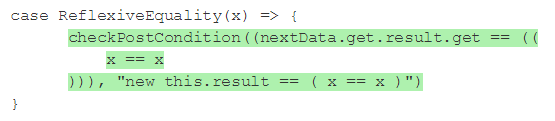
\includegraphics[width=\linewidth]{figures/eval_e0_reflexive-equality}
}
\caption{Test coverage example for \textit{ReflexiveEquality}}
\label{fig:ch3_eval_e0_highlighting_reflexive-equality}
\centering
\end{figure}
\FloatBarrier
% End figure
\pinfo{Property coverage}
The logic of a specification is defined in one Class in the generated system, which is called \textit{Logic} and prefixed by the specification name. We will only look at these classes to check to which extent the properties have been tested, using the highlighting that shows the coverage. This is because our test suit is not intended to check the other components of the system. However, all files in the generated system will be used to determine the overall coverage percentage. Since we use the same SUT to determine the coverage of the test suite on the SUT, the higher the coverage, the more complete it tests the defined properties in the generated system.

% Amount of bugs
\subsubsection{Amount of bugs}
\pinfo{Not a hard criteria, still using for indication}
The number of bugs found by an experiment also describes how effective the experiment was. Although this can not be a hard criteria, as it can vary per case. Consider that the system was already tested thoroughly, such that the bugs that this test suite would have found are already solved. This would mean that the amount of bugs found would remain 0, thus wouldn't have any effect as criteria. It is still an interesting part, as the amount of bugs found proofs that the test suite is able to find bugs. Because of this, we will report on this criteria and take it into account, but it will not be a critical criteria on determining whether one experiment was more successful than the other.

%\todo[inline]{Efficiency? Not yet.\\
%Can be done like getting coverage of libraries too, then substitute amount of properties and show that the same coverage can be received with less property tests. Thus less test cases, faster speed, same coverage. However, this would entail that the amount of bugs could go lower, as certain specific properties wont be tested if we require only coverage.}


% % % % % % % % % % % % % % % % % % % % % % % % % % % % % % % % % % % % %
% Section: Analysis
\section{Analysis}
...

% % % % % % % % % % % % % % % % % % % % % % % % % % % % % % % % % % % % %
% Section: Threats to validity
\section{Threats to validity}
...
